\section{Servidor}

É de notar que até este ponto no relatório se faz referência ao servidor como uma componente.
Nesta secção o servidor é analisado como o conjunto das suas componentes, descrevendo-se as funcionalidades de cada componente, meios de comunicação e protocolo.


\subsection{Broker}

Os brokers do servidor são instâncias de uma aplicação desenvolvida em Ruby. Cada instância difere apenas nos endereços de comunicação, o endereço para comunicação com clientes e outro para comunicação com os restantes brokers.
Sendo que cada broker executa num processo Ruby justifica-se que na mesma máquina se executem diversos brokers de forma a tirar partido de paralelismo de processamento (ver secção~\ref{sec:ruby}).
Note-se que cada broker executa numa thread apenas uma vez que foi desenvolvida no paradigam orientado a eventos fazendo uso da ferramenta EventMachine (ver secção~\ref{sec:eventmachine}).

Toda a comunicação no servidor é realizada por websockets, tanto para os clientes como entre os brokers. Mais detalhes no protocol de comunicação na secção~\ref{sec:protocolo}.

\subsubsection{Componentes}
Cada broker executa dois serviços de websockets:

\begin{itemize}
\item um para comunicação com os clientes. Será identificado ao longo do relatório como \textbf{serviço de comunicação}).
\item um para comunicação com os restantes brokers. Será identificado ao longo do relatório como \textbf{serviço de sincronização}).
\end{itemize}

Note-se que ainda que execute dois serviços de websockets que atendem em portas diferentes existe apenas uma thread por broker.

O serviço de comunicação com os clientes é responsável por toda a comunicação com os clientes. Este servidor responde aos seguintes eventos de um cliente:
\begin{enumerate}
\item \textbf{nova ligação}. O serviço é recolhe o próximo identificador único da base de dados e envia ao cliente. Este identificador serve apenas para o cliente poder assinar as suas mensagens ou reconhecer as mensagens de outro cliente (este identificador não tem utilidade ao servidor).
\item \textbf{subscrição de canal}. O serviço procura o canal ou cria um novo e devolve ao cliente uma mensagem de sucesso.
\item \textbf{remoção da subscrição de um canal}. O serviço remove a subscrição do cliente.
\item \textbf{mensagem para diversos canais}. O serviço difunde a mensam pelos respectivos canais e submete para o serviço de sincronização.
\end{enumerate}

\hl{}

\textbf{Novo servidor}
\begin{enumerate}
\item Iniciar o servidor que recebe ligações dos restantes brokers.
\item Registar o endereço do servidor na base de dado
\item Criar a ligação a todos os brokers que estão activos na base de dados.
\item Utilizar cada ligação para informar da actualização da lista de brokers.
\item Iniciar o servidor de websockets.
\end{enumerate}



\subsection{Arquitectura}

O servidor é composto por um, ou vários, brokers e uma base de dados. Os brokers são instâncias da mesma aplicação, ou seja, são idênticos, e a base de dados é PostgreSQL. A ideia é ser indiferente o broker ao qual um cliente establece ligação uma vez que o comportamento é distribuído pelos restantes.
Por exemplo: dois clientes subescreverem o mesmo canal em brokers diferentes e um terceiro cliente envia uma mensagem para esse canal, então ambos os novos clientes recebem a mensagem.

\begin{figure}[H]
\centering
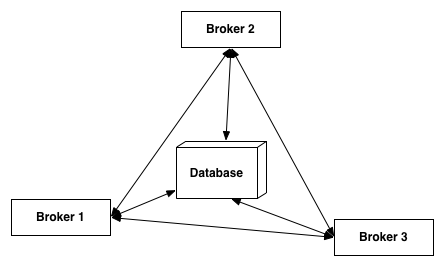
\includegraphics[width=0.65\textwidth]{brokers.png}
\caption{\textit{Visão simplista da arquitectura do servidor.}}
\label{fig:brokers-arq}
\end{figure}

A figura~\ref{fig:brokers-arq} apresenta um esquema simplista das ligações entre os diferentes componentes do servidor. Como se pode ver os brokers estão todos ligados entre si e cada um está ligado à base de dados.
A base de dados é responsável por armazenar as mensagens persistentes, manter uma sequência que forneça identificadores únicos para identificar os clientes e registar os endereços dos servidores activos. Todas as restantes acções são da responsabilidade dos brokers, deste modo a ligação entre todos os brokers serve dois propósitos:

\begin{enumerate}
\item \textbf{Difundir mensagens}. As mensagens que um broker recebe são difundidas pelos restantes. Isto permite que vários clientes possam subscrever os mesmos canais quando estão ligados em brokers diferentes.
\item \textbf{Informar da actualização na lista de servidores}. Quando existe um novo broker online ou um dos brokers é identificado como inactivo o novo broker ou o broker que identificou o problema, respectivamente, actualizam a base de dados e enviam uma mensagem de actualização a todos os brokers.
\end{enumerate}

